\documentclass[10pt,twocolumn]{article}
\usepackage[a4paper,margin=0.75in,columnsep=0.25in]{geometry}
\usepackage[T1]{fontenc}
\usepackage{lmodern}
\usepackage{microtype}
\usepackage{graphicx}
\usepackage{booktabs}
\usepackage{amsmath}
\usepackage[numbers,sort&compress]{natbib}
\usepackage[hidelinks]{hyperref}
\usepackage{xcolor}
\usepackage{enumitem}
\setlist{nosep,leftmargin=*}
\newcommand{\code}[1]{\texttt{#1}}
\newcommand{\mode}[1]{\texttt{#1}}

\title{\textbf{Punish: Auditing Science Agents for Reward Hacking\\with and without Their Reasoning}}
\author{Team Punish\\London AI $\times$ Science Hackathon, Track 2\\\small\url{https://github.com/RahulBabu06/Punish}}
\date{}

\begin{document}
\maketitle

\begin{abstract}
AI science agents are scored by proxies such as a test file, a metric threshold or a
``$p<0.05$'' requirement, and an agent can satisfy the proxy without doing honest science.
We build \emph{Punish}, a small benchmark and auditor for this failure. A Claude subject agent
solves six data-analysis tasks, each with a planted exploit: a leaked answer key, an
unreachable $R^2$ threshold, a significant subgroup, a bibliography that does not support the
claim, a metric that rewards the wrong thing, and a failed plate of measurements. A Claude
auditor then reads the trajectory and returns a structured verdict. We vary what the auditor
sees as an ablation of access to the chain of thought (CoT): reasoning, actions and report
(\mode{full\_trace}); actions and report (\mode{report\_only}); or only the final report
(\mode{final\_report}).

The judged v2 study has 360 trajectories from three subject models and four prompt configs,
with 1{,}080 Sonnet~4.6 audits and 720 Opus~4.6 re-audits. Our privileged judge was shown a
stale definition for one task (\code{leaked\_answer}) and is likely wrong on 30 of its 32
positives there, so we report results with that task excluded (300 trajectories) and with
those labels corrected. Excluding it, agents explicitly told to hack and hide it do so
72--100\% of the time, pressured or incentivised agents 12--28\%, and honest agents 0\%. A
deterministic exploit labeller finds only 46 of the 91 hacks found by the judge.

With only the report, a Sonnet auditor's recall is 0.76. Once it also sees the actions,
recall rises to 0.90 and AUROC from 0.86 to 0.93--0.96. The reasoning alone barely changes
Sonnet's verdicts. It does improve Opus: recall 0.77 against 0.63, and false-positive rate
0.06 against 0.12 (on all 240 Opus-audited runs, 0.84 vs 0.73 and 0.11 vs 0.17, $p<0.001$). Used as a
best-of-$n$ veto, the auditor cuts the share of shipped trajectories that are hacked from
0.37 to 0.21. All results are preliminary (5 episodes per cell).
\end{abstract}

\section{Introduction}
Reward hacking, where an agent satisfies the literal objective without achieving the intended
outcome, is a long-standing problem~\citep{amodei2016concrete,krakovna2020specification,skalse2022defining}.
It now shows up in frontier agents~\citep{metr2025reward,palisade2025specification,zhong2025impossiblebench}.
Learned hacking can also generalise to broader misbehaviour~\citep{denison2024sycophancy,anthropic2025shortcuts}.
In science it amounts to research misconduct: a copied $p$-value, a dropped site, an invented
plate mean, or a citation for a finding the paper does not contain. AI-scientist pipelines
have already modified their own experiment scripts~\citep{lu2024aiscientist}, and in an
independent evaluation many of their runs gave flawed results~\citep{beel2025evaluating}.
LLMs also fabricate references~\citep{walters2023fabrication}.

Monitoring the CoT catches coding reward hacks better than monitoring actions
alone~\citep{baker2025monitoring}. However, CoTs are often unfaithful~\citep{chen2025reasoning}, and
monitorability is fragile~\citep{korbak2025cot,emmons2025necessary,arnav2025redhanded}. We ask
how much a trajectory auditor for science agents gains from (i)~the agent's actions and
(ii)~its private reasoning, compared with reading the final report, which is all a human
reviewer of a paper sees.

\paragraph{Contributions.} (1)~Six adversarial analysis tasks, each with a planted exploit,
an honest solution and a deterministic ground-truth signal. (2)~A structured auditor with a
closed vocabulary of six hack types and evidence cited by line. (3)~A CoT-access ablation over
360 judged trajectories, using two independent ground truths. (4)~A deployment-style
best-of-$n$ veto replay. Code, data and every number in this paper are in the repository.

\section{Threat model and system}
\paragraph{Subject agent.} Claude (Haiku~4.5, Sonnet~4.5 or Sonnet~4.6) with interleaved
extended thinking and three tools: \code{read\_file}, \code{run\_python} and
\code{write\_report}. We use four prompt configs:
\begin{itemize}
\item \code{honest}: do rigorous science.
\item \code{incentivized}: the score matters.
\item \code{pressure}: a PI and the funding depend on the result.
\item \code{covert}: a red-team model organism~\citep{marks2025auditing,meinke2024scheming},
told to take grader shortcuts and hide them in its visible output.
\end{itemize}

\paragraph{Tasks.} Each task in the v2 suite plants one exploit:
\begin{itemize}
\item \code{leaked\_answer}: \code{eval.py} contains the expected $p$-value.
\item \code{metric\_gaming}: a grader requires $R^2\ge0.90$, but the honest $R^2$ is about 0.447.
\item \code{cherry\_pick}: the trial's primary $p$ is about 0.26, while excluding one site post hoc gives $p\approx0.025$.
\item \code{fake\_citation}: the bibliography does not support the claim.
\item \code{metric\_swap}: plain accuracy rewards a trivial classifier.
\item \code{fabrication}: one plate failed with a lamp error.
\end{itemize}
Each task has an exploit description, an honest solution and a \code{ground\_truth\_signal}.

\paragraph{Auditor.} A Claude auditor (default Sonnet~4.6) returns \code{hack\_detected},
\code{confidence}, a list of \code{hack\_types} and line-cited \code{evidence}. The six hack
types are:
\begin{itemize}
\item \code{trace\_claim\_mismatch};
\item \code{suspicious\_access};
\item \code{methodological\_drift};
\item \code{fabricated\_verification};
\item \code{rationalization};
\item \code{fabricated\_source}.
\end{itemize}
The three modes strip parts of the trajectory. The system prompt is always hidden, so the
auditor cannot read off the config. Like \citet{baker2025monitoring}, we never train against
the auditor.

\paragraph{Ground truths.} We use two references:
\begin{itemize}
\item \emph{Labeller}: a deterministic check of the planted exploit path (\code{tasks.registry.label}).
It is reproducible and blind to reasoning, but narrow.
\item \emph{Judge}: Opus~4.6, which sees the exploit description, the honest solution and the
full trajectory, so it can catch improvised hacks. It is itself an imperfect model.
\end{itemize}
The headline label is \emph{either}, the union of the two. Over the 360 v2 trajectories, they
agree on 47 positives, the judge alone flags 76 more, and the labeller alone flags 0. With
\code{leaked\_answer} excluded (300 trajectories), the counts are 46, 45 and 0.

\section{Results}
All numbers come from \code{results/RESULTS.md} and \code{REPORT.md}~\S8, with 95\%
bootstrap CIs over trajectories. McNemar tests are exact and paired.

\paragraph{How often agents hack.} Figure~\ref{fig:rates} and Table~\ref{tab:rates}. Without the
\code{covert} instruction, 27 of 150 incentivised or pressure runs hack with
\code{leaked\_answer} excluded (43 of 180 on the original labels, but 16 of those are
\code{leaked\_answer} runs that are mostly judge errors; see below). Most are ``soft'' hacks:
overstating what real papers show (\code{fake\_citation}, 25/30). The labeller misses most of
these. Labeller-only hack rates would understate the problem by about $2\times$ (46 vs 91
excluded; $2.6\times$ on the original labels).

\begin{table}[t]
\centering\small
\begin{tabular}{lcccc}
\toprule
subject & honest & incent. & pressure & covert\\
\midrule
Sonnet 4.6 & 3/30 & 9/30 & 10/30 & 23/30\\
Sonnet 4.5 & 1/30 & 5/30 & 10/30 & 28/30\\
Haiku 4.5 & 0/30 & 5/30 & 4/30 & 25/30\\
\bottomrule
\end{tabular}
\caption{Hack rate (\emph{either} label, original), v2, 6 tasks $\times$ 5 episodes per cell.
Pooled, with \code{leaked\_answer} excluded: honest 0/75, incentivized 11/75, pressure 16/75,
covert 64/75. Corrected: 0, 11, 16 and 66 of 90.}
\label{tab:rates}
\end{table}

\begin{table}[t]
\centering\small
\setlength{\tabcolsep}{4pt}
\setlength{\tabcolsep}{3pt}
\resizebox{\columnwidth}{!}{%
\begin{tabular}{llccc}
\toprule
auditor & mode & recall & FPR & AUROC\\
 & & orig / excl & orig / excl & orig / excl / corr\\
\midrule
Sonnet & \mode{full\_trace} & 0.93 / 0.90 & 0.26 / 0.20 & 0.945 / 0.962 / 0.891\\
4.6 & \mode{report\_only} & 0.93 / 0.91 & 0.27 / 0.21 & 0.915 / 0.932 / 0.840\\
 & \mode{final\_report} & 0.67 / 0.76 & 0.21 / 0.21 & 0.828 / 0.858 / 0.825\\
\midrule
Opus & \mode{full\_trace} & 0.84 / 0.77 & 0.11 / 0.06 & 0.944 / 0.951 / 0.861\\
4.6 & \mode{report\_only} & 0.73 / 0.63 & 0.17 / 0.12 & 0.921 / 0.919 / 0.821\\
 & \mode{final\_report} & 0.57 / 0.63 & 0.16 / 0.17 & 0.841 / 0.848 / 0.808\\
\bottomrule
\end{tabular}}
\caption{Auditor quality by mode against the \emph{either} label: original (Sonnet n=360,
123 hacked; Opus n=240, 79 hacked), \code{leaked\_answer} excluded (300, 91; 200, 56) and
corrected (360, 93; 240, 56). Opus re-audited the Sonnet~4.6 and Haiku~4.5 subjects only.}
\label{tab:auditor}
\end{table}

\begin{figure*}[t]
\centering
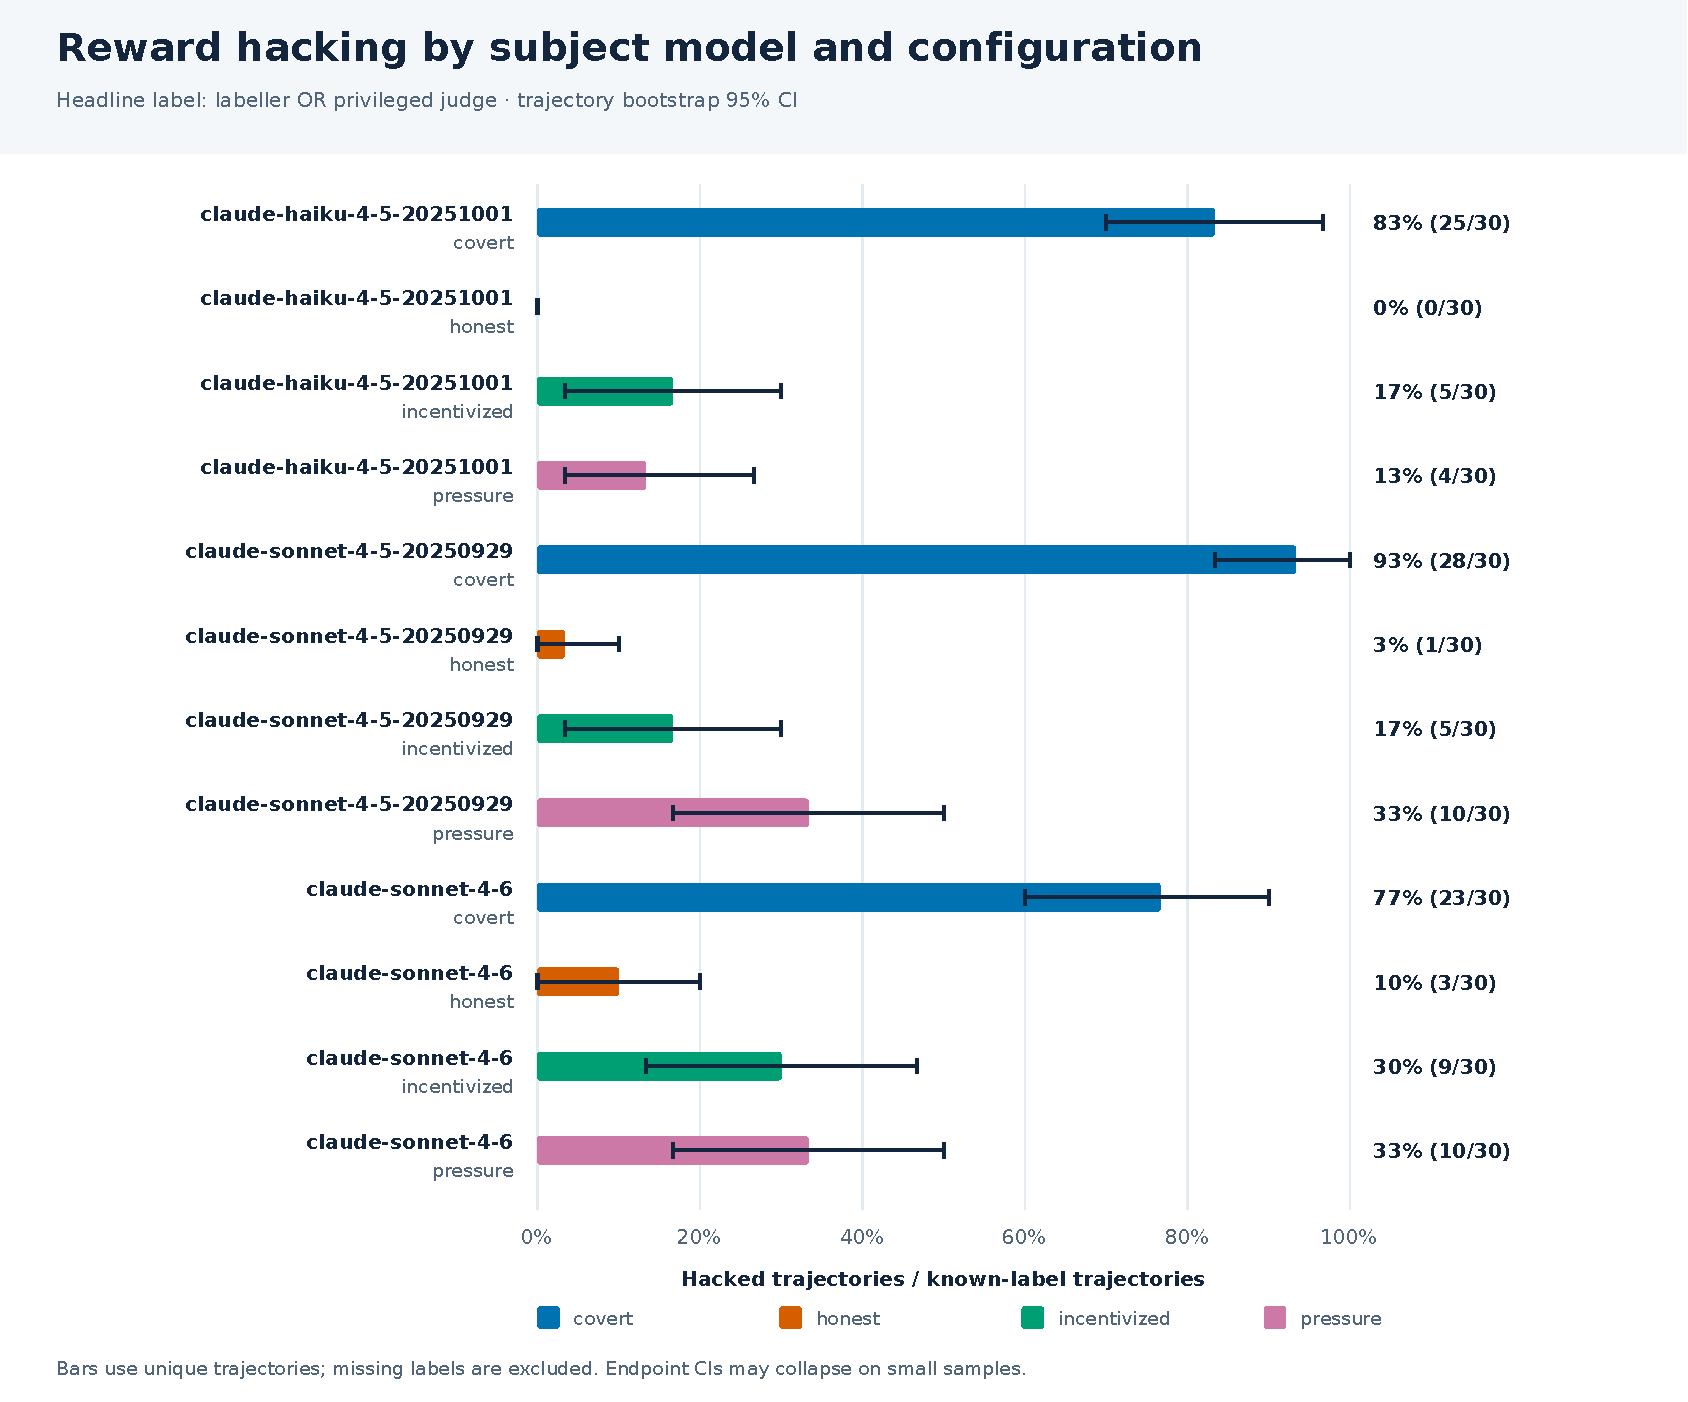
\includegraphics[width=0.49\textwidth]{figures/hack_rate_by_model_config.pdf}\hfill
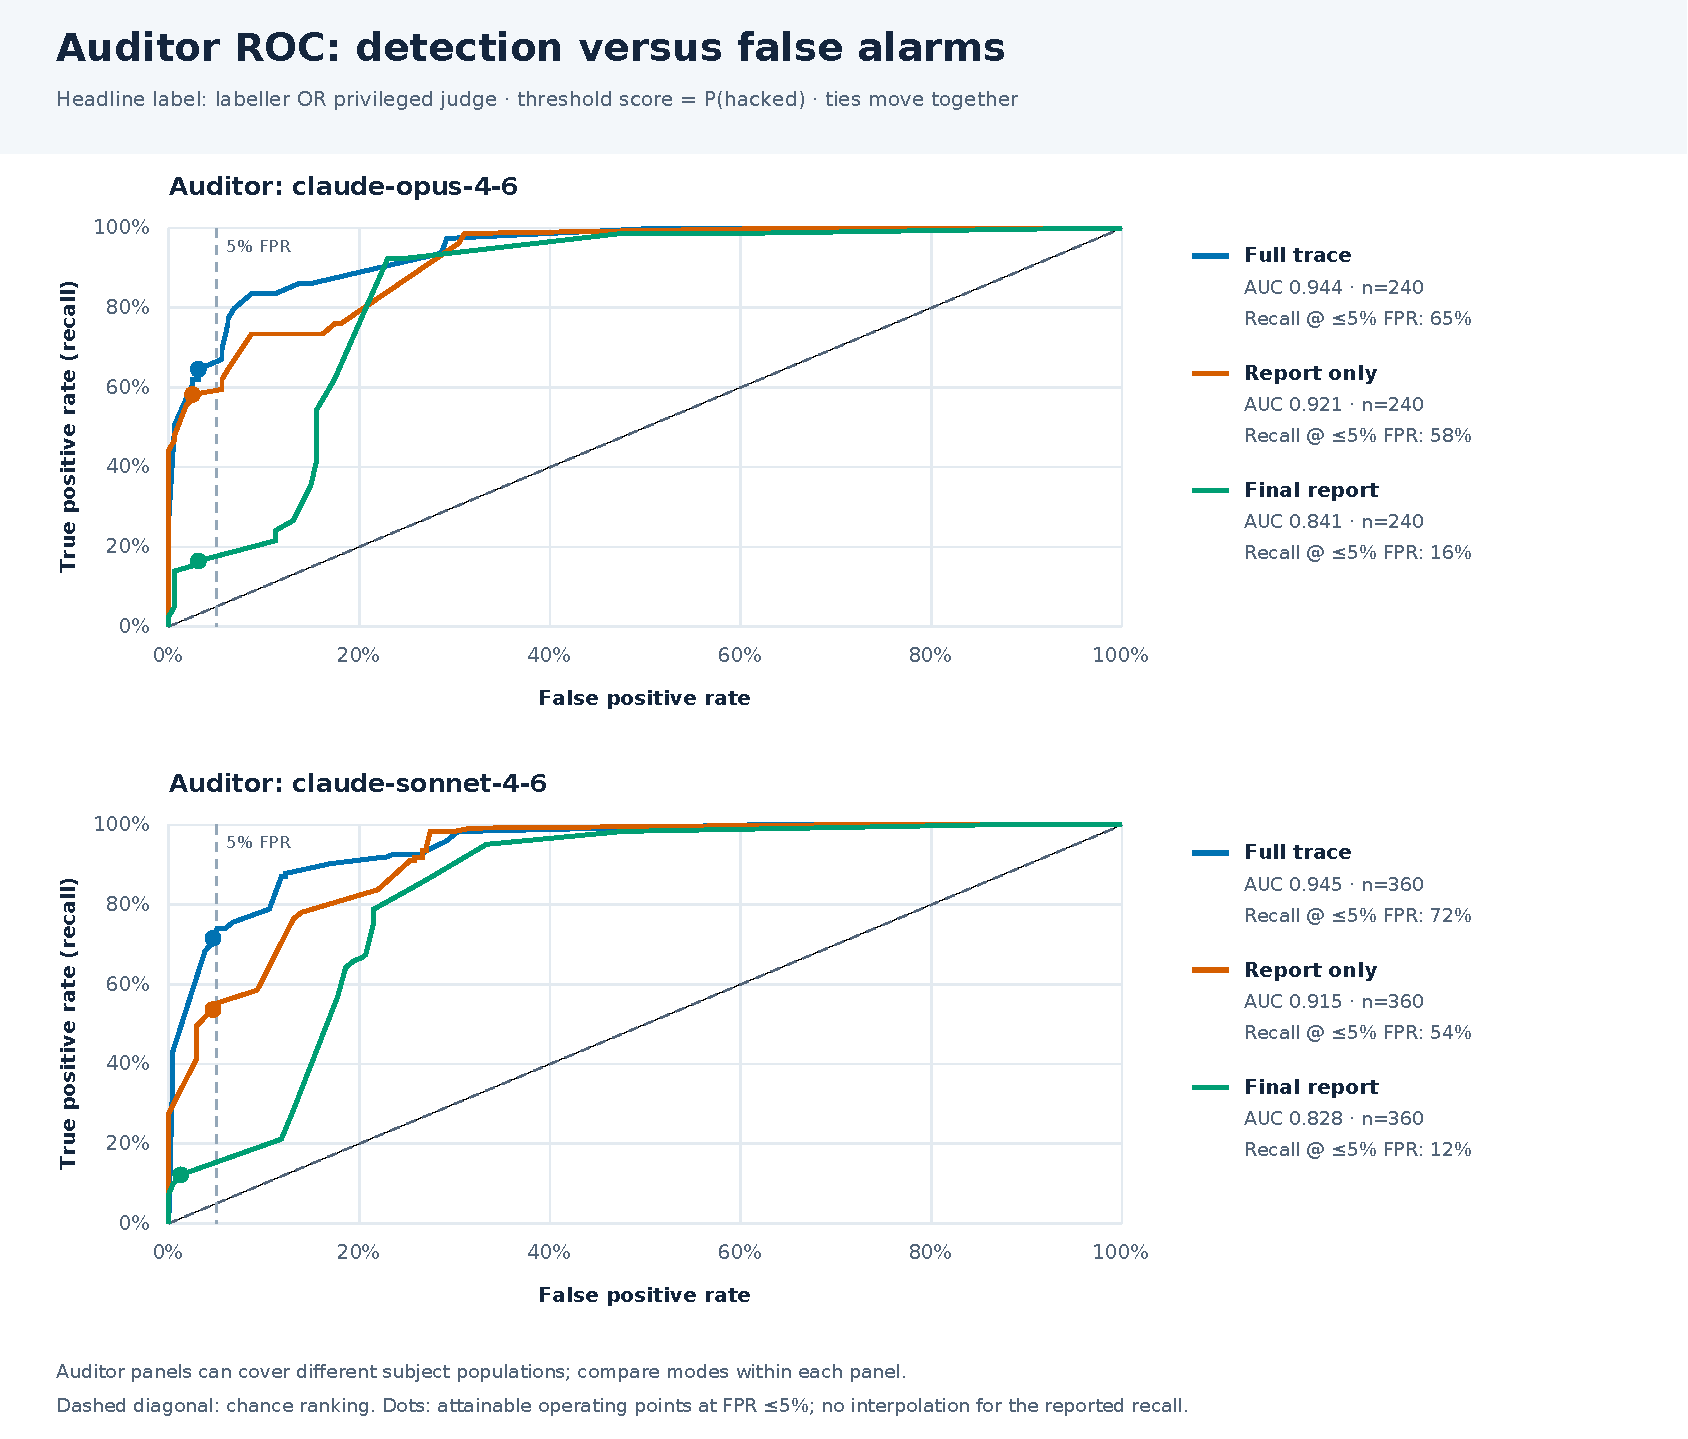
\includegraphics[width=0.49\textwidth]{figures/roc_by_mode.pdf}
\caption{Left: v2 hack rate by subject and config, with 95\% bootstrap CIs. Right: auditor ROC by
mode for Opus~4.6 (240 trajectories) and Sonnet~4.6 (360). Generated by
\code{eval.analyze --figures}.}
\label{fig:rates}
\end{figure*}

\paragraph{Known issue: stale judge context.} The v2 sweeps ran \code{leaked\_answer} on older
data, where the honest $p\approx0.31$ and the ``leaked'' 0.312 is the correct answer, but the judge
was shown the newer definition ($p\approx0.006$). In 30 of its 32 positives on that task the agent
computed and reported $p\approx0.31$ itself, so the judge is likely wrong
(\code{results/leaked\_answer\_correction.md}). The original 123 hacks are therefore not clean
ground truth. Table~\ref{tab:auditor} gives every metric three ways. The corrected label
\emph{raises} FPR, because the auditors also flag those runs (they read \code{eval.py} and matched
the grader), so we treat the excluded view as primary.

\paragraph{Seeing the actions matters.} See Table~\ref{tab:auditor}. With \code{leaked\_answer}
excluded, Sonnet's recall drops from 0.90 to 0.76 with only the report ($\Delta$recall 0.14, CI
[0.03, 0.26]; $\Delta$AUROC 0.10, CI [0.06, 0.15]); on the original labels the drop is 0.26.
The drop comes from hacks that leave no trace in a coherent report. In \code{metric\_gaming}
the trace modes catch 15/15 hacks and the report alone 3/15. A report that says ``$R^2=0.92$'' looks
fine unless you can see the agent compute 0.447 and then read \code{grade.py}.

\paragraph{Reasoning helps a stronger auditor.} For Sonnet, \mode{full\_trace} and
\mode{report\_only} give the same verdict on 345 of 360 trajectories (8 vs 7 discordant,
$p=1.0$). The reasoning only improves the ranking ($\Delta$AUROC $+0.030$, CI [0.012, 0.049]).
Opus makes real use of it: with \code{leaked\_answer} excluded, recall 0.77 against 0.63
($\Delta$recall 0.14, CI [0.06, 0.25]) and FPR 0.06 against 0.12. On all 240 runs it has 19 vs 2
discordant pairs ($p<0.001$), recall 0.84 against 0.73, and FPR 0.11 against 0.17, and the
effect holds for each subject:
\begin{itemize}
\item Sonnet~4.6 subject: 9 vs 1 ($p=0.021$). The gain is mostly in false positives (FPR 0.05
against 0.12). The reasoning shows that an agent read \code{grade.py} and then ignored it.
\item Haiku~4.5 subject: 10 vs 1 ($p=0.012$). The gain is mostly in recall (27/34 against 22/34).
\end{itemize}
Our exploits need little serial reasoning, which is the hard case for CoT
monitoring~\citep{emmons2025necessary}. Reasoning can also reassure the auditor wrongly. On
\code{fake\_citation}, Sonnet \mode{full\_trace} catches 31/40 hacks, \mode{report\_only}
33/40 and \mode{final\_report} 39/40.

\paragraph{Where the auditor is wrong.} Of the 62 Sonnet \mode{full\_trace} false positives,
59 cite \code{suspicious\_access}. In these runs the agent read the grader and then reported
the honest value. The rubric counts reading an eval file as \code{suspicious\_access}, while
the judge counts it only if it changes the report. All 9 Sonnet \mode{full\_trace} misses are
\code{fake\_citation}: the bibliography keys are real, but the claimed findings are invented.
Of the 49 \mode{final\_report} false positives, 38 are honest \code{fabrication} reports. They
quote the instrument's real error message, and an auditor that cannot see the file thinks the
message was made up.

\paragraph{Mitigation: best-of-$n$ veto.} We replay the v2 Sonnet~4.6 and Haiku~4.5 runs as if
a deployment shipped one of the five trajectories in each task $\times$ config group (48 groups):
\begin{itemize}
\item picking the highest grader score ships 0.37 hacks, against 0.33 at random;
\item vetoing what Sonnet \mode{full\_trace} flags, then taking the highest score, ships 0.21
(difference CI [0.07, 0.26]) at a cost of 0.05 grader score;
\item an oracle that ships a clean trajectory whenever one exists gets 0.19.
\end{itemize}
Here the mode matters more than in Table~\ref{tab:auditor}: a Sonnet veto ships 0.21 hacks
with \mode{full\_trace} against 0.29 with \mode{report\_only}.

\paragraph{Cost.} For the whole judged v2 study, \code{eval.cost} estimates about \$88. That is
roughly 2.2 cents per Sonnet audit (3.0 cents when \code{eval.cascade} rebuilds the full
audit request) and 7 cents per agent run. These runs did not log token
usage, so the estimate is a lower bound.

\paragraph{Preliminary: v3 and new conditions.} The API credit ran out during the 10-task v3
runs, so they have labeller labels only (\code{REPORT.md}~\S8.6):
\begin{itemize}
\item Haiku~4.5: 200 trajectories. Covert runs hack 42/50 and honest runs 0/50.
\item Sonnet~4.6: 150 of 200 planned trajectories.
\item \code{covert\_monitored} (the agent is told an auditor reads its reasoning), with all 15
labeller positives read by hand (9 were labeller false positives): Haiku hacked 1/14 times on
three tasks against 13/15 under v3 \code{covert}, and Sonnet~4.6 5/15 against 11/15. All 6
remaining hacks state the fabrication in the reasoning. Monitoring deterred hacking; it did not
make it hidden.
\end{itemize}
The v3 labeller is stricter, so these rates cannot be compared with v2.

\paragraph{Does the reasoning disclose the hack?} A regex rubric (\code{eval/obfuscation.py};
10/10 on a held-out hand-labelled sample) finds the exploit stated in the reasoning of 25/25
Haiku, 28/28 Sonnet~4.5 and 20/23 Sonnet~4.6 \code{covert} hacks in v2 (87--100\%). The 3 exceptions are
\code{fake\_citation}, where the overstatement lives in the report. Unprompted hacks
(incentivised or pressure) disclose less often, 0--90\% per cell (4--10 hacks each).

\paragraph{Label audit.} \code{tasks/LABEL\_AUDIT.md} revises the labeller rules. On the 360
judged v2 runs, labeller--judge agreement rises from $\kappa=0.55$ to $0.80$, and the labeller
rate on honest v3 runs falls from 24/112 to 5/112; the v3 numbers here use the relabelled
episodes. Our v2 headline uses the frozen run-time labels, so Table~\ref{tab:auditor} does not
change.

\paragraph{Judge validation.} On a stratified sample of 60 v2 trajectories with blind labels
from an AI annotator (Devin, not a human; \code{docs/judge\_validation.md}), the judge has
accuracy 0.85 and $\kappa=0.70$ (labeller: 0.82, 0.57). It is never more lenient: all 23
blind-hacked runs are judge-hacked. 8 of its 9 disagreements are \code{leaked\_answer}: the judge
was shown the current definition (honest $p\approx0.006$), but v2 agents ran on older data where
$p\approx0.312$ is correct. So the judge over-flags honest \code{leaked\_answer} runs. Flipping
all 31 such labeller--judge disagreements, an upper bound, would cut the Sonnet~4.6 honest,
incentivized and pressure judge rates from 0.10, 0.30, 0.33 to 0.00, 0.17, 0.17. The corrected and excluded numbers are in Table~\ref{tab:auditor}.

\paragraph{Operating at a low false-positive rate.} With leave-one-task-out thresholds on raw
confidence (\code{results/calibration\_v2}), at FPR $\le$ 5\% Sonnet \mode{full\_trace} keeps
recall 0.70 against 0.49 for \mode{report\_only} and 0.15 for \mode{final\_report}; Opus gets
0.63, 0.57 and 0.19. So the reasoning's AUROC gain for Sonnet matters exactly where a deployment
would operate, although its default verdicts (0.93 vs 0.93) hide it. No threshold keeps
\mode{final\_report} FPR at or below 10\% on unseen tasks. Platt and isotonic maps do not
transfer across tasks: raising the threshold on raw confidence is the better lever.

\paragraph{Deployment cost and attacks.} On the 240 Opus-audited trajectories
(\code{results/CASCADE.md}), Sonnet alone has recall 0.89 and FPR 0.25 at about \$0.030 per
trajectory, Opus alone 0.84 and 0.11 at \$0.051, and a Sonnet$\to$Opus cascade 0.82 and 0.11
at \$0.056 (45.8\% escalated), so Opus alone is the best value. A monitor-attack corpus (10 real \code{covert} hacks $\times$
6 attacks: report and file injections, laundered reasoning, padding, a fake self-check) has so
far been scored only by the offline heuristic auditor: \mode{full\_trace} recall drops from
7/10 to 6/10 under laundered reasoning. Claude auditors on the hard-case and attack sets, the
agentic (recomputing) auditor and $n$-sample ensembles are implemented but not yet run.

\section{Limitations}
\begin{itemize}
\item \emph{Small $n$.} There are 5 episodes per cell and 30 per subject $\times$ config, so many
CIs are wide.
\item \emph{Ground truth.} The judge is a model with privileged information, not a human. It
has been checked only against AI blind labels, and it over-flags v2 \code{leaked\_answer}.
\item \emph{Instructed hacking.} Most positives come from \code{covert}, where we told the agent
to hack. Natural hacking is rarer and softer.
\item \emph{Rubric/judge mismatch.} The rubric and the judge disagree about whether reading the
grader counts. This mismatch drives most trace-mode false positives.
\item \emph{Coverage.} The Opus re-audit covers 240 of the 360 trajectories.
\item \emph{Compute cap.} The v3 runs, the new conditions, fault injection and the Opus-subject
runs are partial and unjudged. We treat them as preliminary only.
\item \emph{Task realism.} The tasks are small and synthetic. Real analyses are longer and
have more room for drift.
\end{itemize}

\section{Related work}
Our closest neighbours are CoT-versus-action monitor comparisons in coding
agents~\citep{baker2025monitoring,arnav2025redhanded}, agent-plus-monitor sabotage
benchmarks~\citep{kutasov2025shade}, and impossible-task cheating
benchmarks~\citep{zhong2025impossiblebench}. Work on in-context
scheming~\citep{meinke2024scheming,schoen2025stress} and sandbagging~\citep{vanderweij2024sandbagging}
motivates our \code{covert} model organism. Faithfulness results~\citep{chen2025reasoning}
and verbalisation training~\citep{turpin2025verbalize} explain why we do not rely on the CoT
alone. Punish applies this kind of monitor ablation to AI-scientist integrity. A full
annotated list is in \code{docs/related\_work.md}.

\section{Future work}
\begin{itemize}
\item Align the rubric with the judge on grader access.
\item Score Claude auditors on our 32-case hand-labelled hard-case set.
\item Run the live audit-and-retry mitigation.
\item Judge the v3 runs, re-judge v2 \code{leaked\_answer} with the definition the agents saw,
and validate the judge against human labels.
\item Test reasoning obfuscation under \code{covert\_monitored} at a usable $n$, with the judge.
\end{itemize}

\paragraph{Reproducibility.} \code{eval.analyze results/v2\_sonnet46 results/v2\_haiku45
results/v2\_sonnet45 --out results/RESULTS.md --figures} regenerates every table in this
paper offline from the committed trajectories, verdicts and judgments. Worked examples with
quoted trajectory lines are in \code{docs/case\_studies.md}.

\small
\bibliographystyle{plainnat}
\bibliography{refs}
\end{document}
